
%(BEGIN_QUESTION)
% Copyright 2008, Tony R. Kuphaldt, released under the Creative Commons Attribution License (v 1.0)
% This means you may do almost anything with this work of mine, so long as you give me proper credit

Determine the amount of time needed after switch closure for the capacitor voltage ($V_C$) to reach the specified levels:

$$\includegraphics[width=15.5cm]{i03246x01.eps}$$

% No blank lines allowed between lines of an \halign structure!
% I use comments (%) instead, so that TeX doesn't choke.

$$\vbox{\offinterlineskip
\halign{\strut
\vrule \quad\hfil # \ \hfil & 
\vrule \quad\hfil # \ \hfil \vrule \cr
\noalign{\hrule}
%
% First row
$V_C$ & Time  \cr
%
\noalign{\hrule}
%
% Second row
0 volts &  \cr
%
\noalign{\hrule}
%
% Third row
10 volts &  \cr
%
\noalign{\hrule}
%
% Fourth row
20 volts &  \cr
%
\noalign{\hrule}
%
% Fifth row
30 volts &  \cr
%
\noalign{\hrule}
} % End of \halign 
}$$ % End of \vbox

\vfil 

\underbar{file i03246}
\eject
%(END_QUESTION)





%(BEGIN_ANSWER)

This is a graded question -- no answers or hints given!
 
%(END_ANSWER)





%(BEGIN_NOTES)

% No blank lines allowed between lines of an \halign structure!
% I use comments (%) instead, so that TeX doesn't choke.

$$\vbox{\offinterlineskip
\halign{\strut
\vrule \quad\hfil # \ \hfil & 
\vrule \quad\hfil # \ \hfil \vrule \cr
\noalign{\hrule}
%
% First row
$V_C$ & Time  \cr
%
\noalign{\hrule}
%
% Second row
0 volts & 0 ms \cr
%
\noalign{\hrule}
%
% Third row
10 volts & 297.5 ms \cr
%
\noalign{\hrule}
%
% Fourth row
20 volts & 716.7 ms \cr
%
\noalign{\hrule}
%
% Fifth row
30 volts & 1.433 s \cr
%
\noalign{\hrule}
} % End of \halign 
}$$ % End of \vbox

%INDEX% Electronics review: RC circuit time constant calculations

%(END_NOTES)


